\documentclass[12pt]{article}
\usepackage[letterpaper, margin=1in, headheight=105pt]{geometry}
\usepackage{subcaption}
\usepackage{graphicx}
\usepackage{hyperref}
\usepackage{pdfpages}
\usepackage{amsmath}
\usepackage{amssymb}
\usepackage{comment}
\usepackage{minted}
\usepackage{pgffor}
\usemintedstyle{manni}

\begin{document}

\section{Homework}

\subsection{Overfitting}
\begin{figure}[htbp]
    \centering
    \begin{subfigure}[t]{0.6\textwidth}
        \centering
        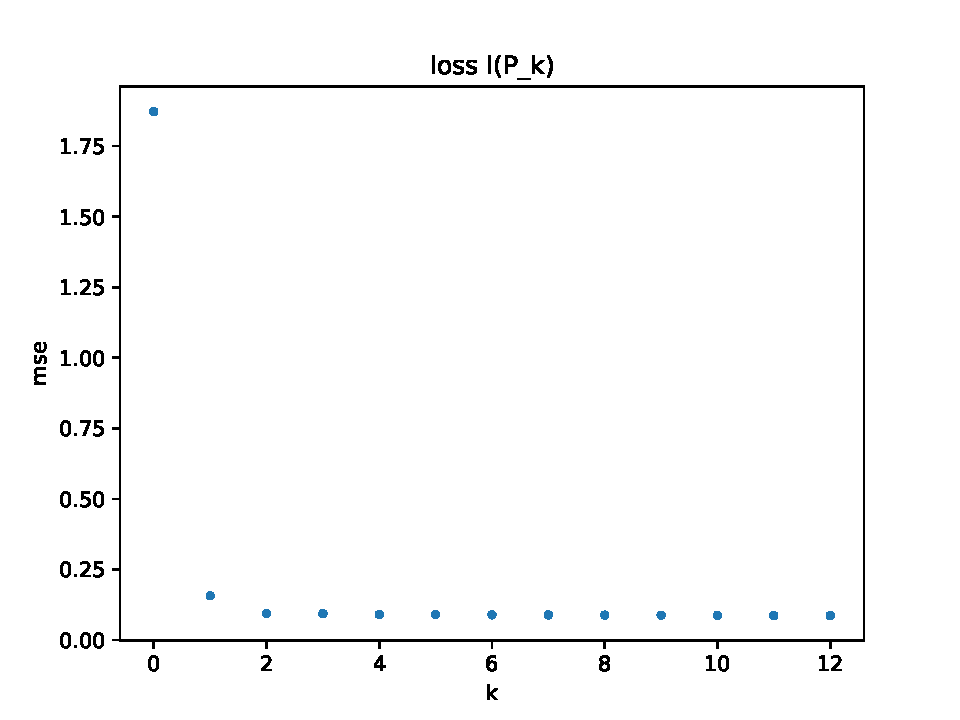
\includegraphics[width=\textwidth]{Homework1/ex1a.pdf}
        \caption{loss \(\ell(\hat{P}_k)\) as a function of \(k\)}
    \end{subfigure}\vspace{10pt}
    \begin{subfigure}[t]{0.6\textwidth}
        \centering
        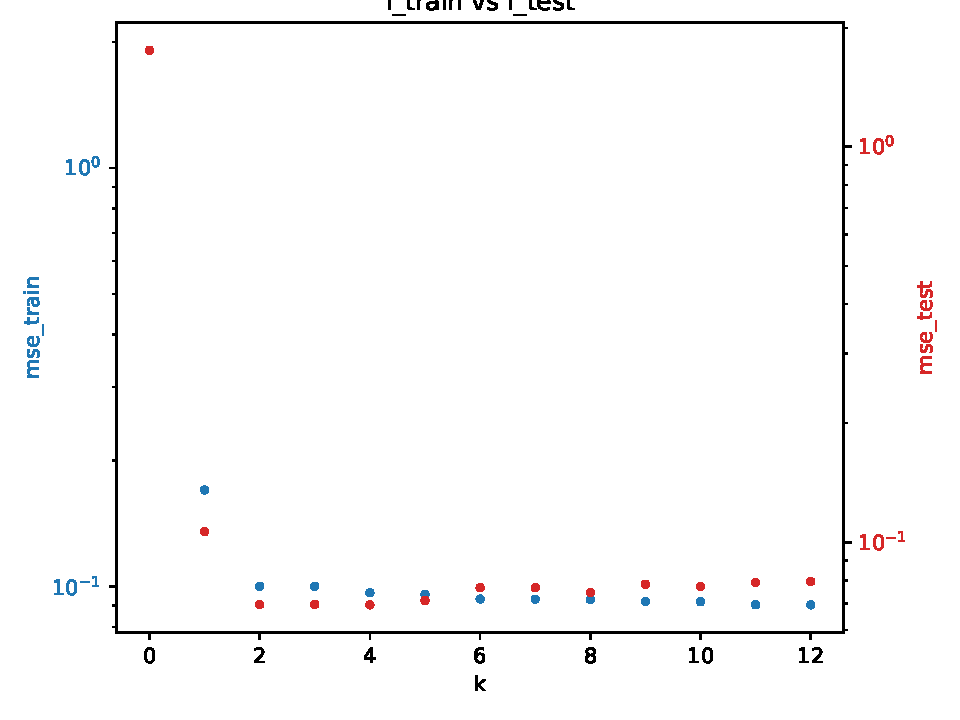
\includegraphics[width=\textwidth]{Homework1/ex1b.pdf}
        \caption{\(\ell_{train}(\hat{P}_k)\) vs \(\ell_{test}(\hat{P}_k)\)}
    \end{subfigure}
\end{figure}
By our observation, \(k_*=2\), and the coefficients are
\[ [a_0, a_1, a_2] = \begin{bmatrix} 0.35333775 & -0.27947762 & 0.81043897\end{bmatrix}. \]
\begin{figure}[htbp]
    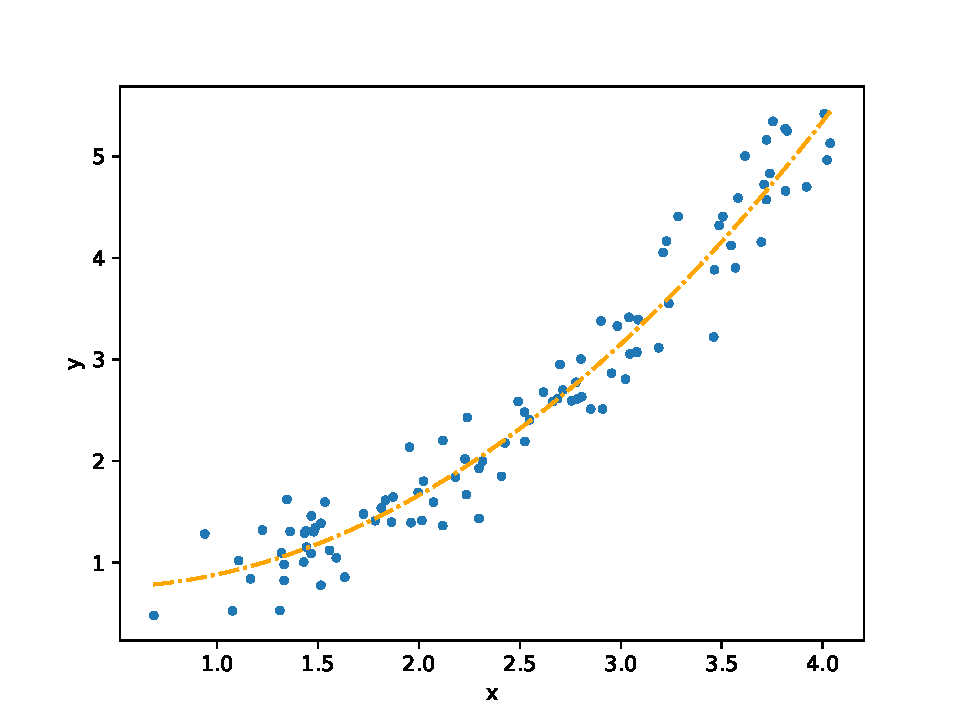
\includegraphics{Homework1/ex1c.pdf}
    \caption{Fitted polynomial by least-square linear regression}
\end{figure}
\inputminted[]{python}{./Homework1/ex1.py}

\subsection{Gradient descent}
\paragraph{(a)}
The loss function can be expanded as
\[ \ell(a,b)= a^2 + b^2\overline{x^2}+ \overline{y^2} + 2ab\overline{x} - 2a\overline{y} - 2b \overline{xy} \]
The gradient of the loss functioin is
\[ \nabla\ell(a,b) = 2\begin{bmatrix}
    a+b\overline{x}-\overline{y} \\
    b\overline{x^2}+a\overline{x}-\overline{xy}
\end{bmatrix} \]
So the minimum is attained at
\[ \begin{bmatrix} a_* \\ b_* \end{bmatrix} = \left(\overline{x^2}-\overline{x}^2 \right)^{-1} \begin{bmatrix}
    \overline{x^2}\cdot\overline{y} - \overline{x}\cdot\overline{xy} \\
    \overline{xy} - \overline{x}\cdot\overline{y} \end{bmatrix}
    \approx \begin{bmatrix}  -1.11233301 \\ 1.48321421 \end{bmatrix} \]
The convergence rate of gradient descent is
\[ \lim_{n\to\infty}\frac{\|(a_n,b_n)-(a_*,b_*)\|}{\|(a_{n-1},b_{n-1})-(a_*,b_*)\|}\approx0.99 \]
\begin{figure}[htbp]
    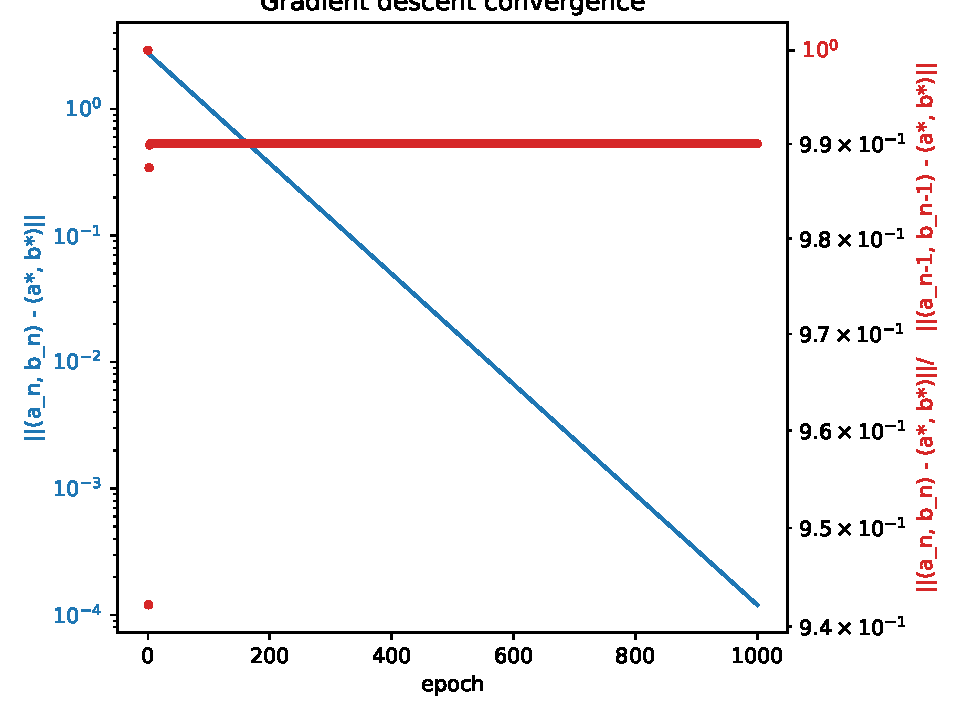
\includegraphics{Homework1/ex2b.pdf}
    \caption{Gradient descent convergence}
\end{figure}
The convergence rate of momentum and Nesterov methods are hard to find on the plot, but they are faster than regular gradient descent.
It takes around 600 epochs to converge to \(10^{-15}\) float-point accuracy, while regular gradient descent takes 1000 epochs to reach \(10^{-4}\).
\begin{figure}[htbp]
    \centering
    \begin{subfigure}[t]{0.68\textwidth}
        \centering
        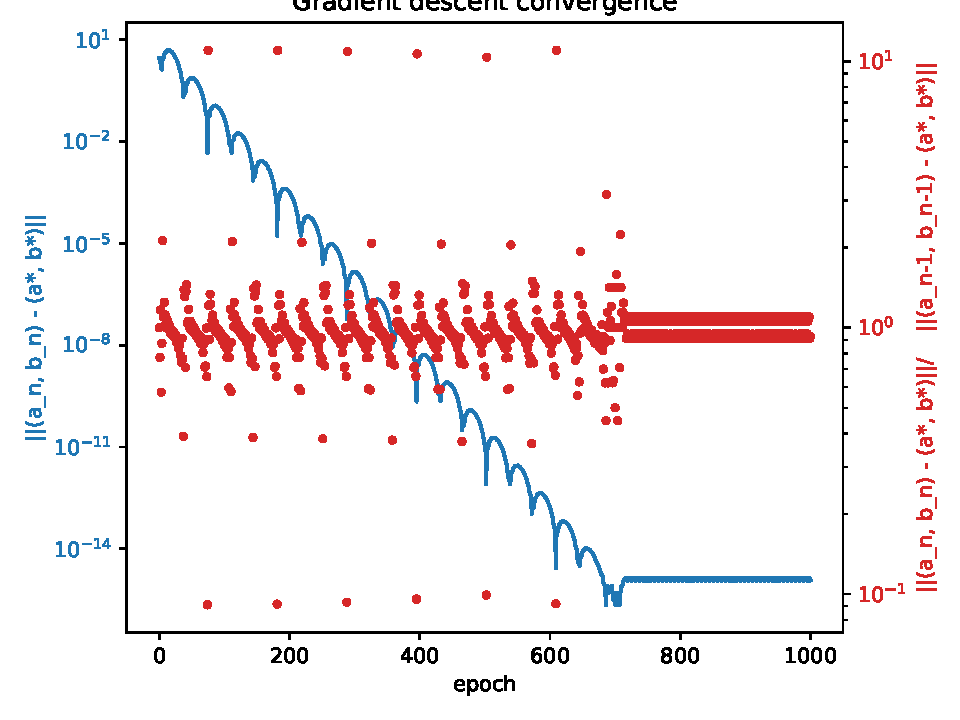
\includegraphics[width=\textwidth]{Homework1/ex2cm.pdf}
        \caption{Convergence of momentum method}
    \end{subfigure}\vspace{10pt}
    \begin{subfigure}[t]{0.68\textwidth}
        \centering
        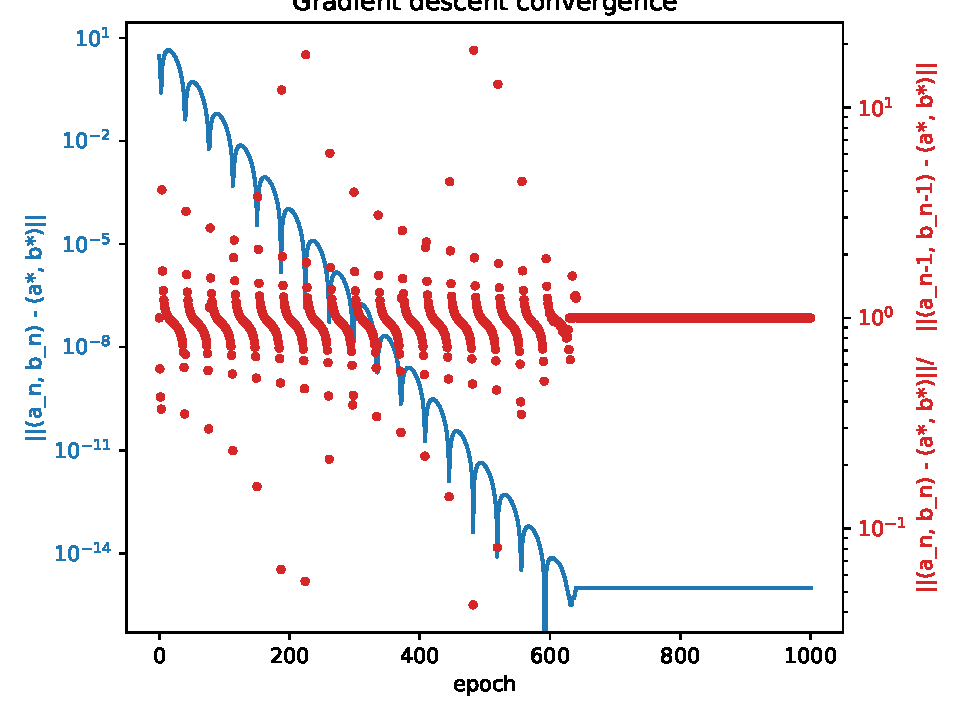
\includegraphics[width=\textwidth]{Homework1/ex2cn.pdf}
        \caption{Convergence of Nesterov method}
    \end{subfigure}
\end{figure}
\paragraph{(extra)}
Other gradient descent methods are implemented in PyTorch.
Most of the errors don't decay as fast as the regular gradient descent.
This is because they are designed for highly non-convex loss functions (to escape from local optimum), while the MSE loss function for linear regression is convex.
\begin{figure}[htbp]
    \centering
    \begin{subfigure}[t]{0.48\textwidth}
        \centering
        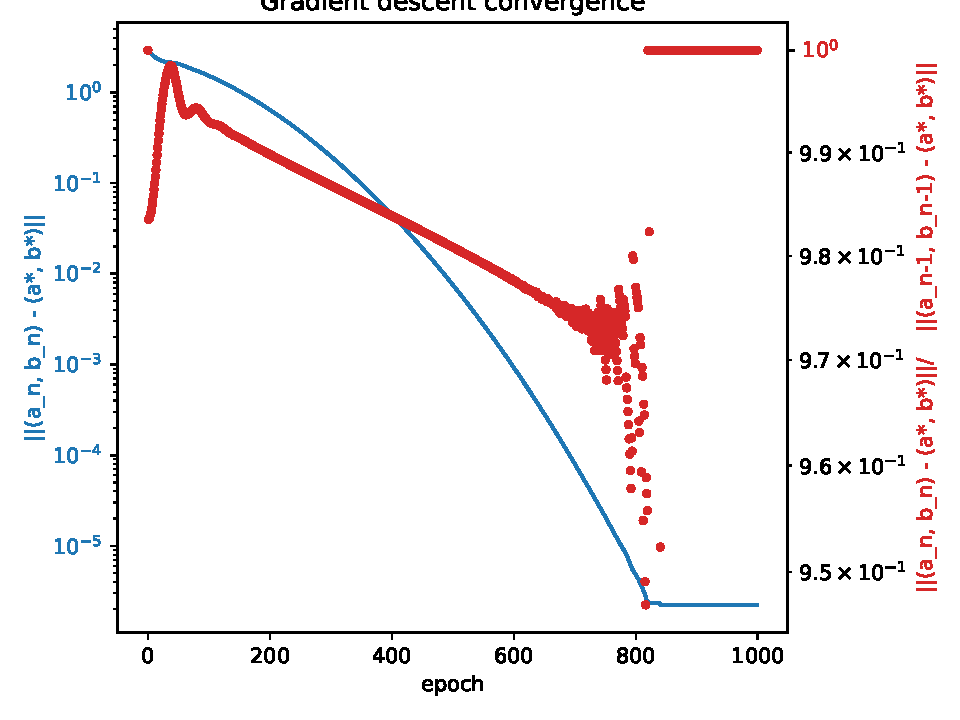
\includegraphics[width=\textwidth]{Homework1/ex2x1.pdf}
        \caption{Adam}
    \end{subfigure}
    \begin{subfigure}[t]{0.48\textwidth}
        \centering
        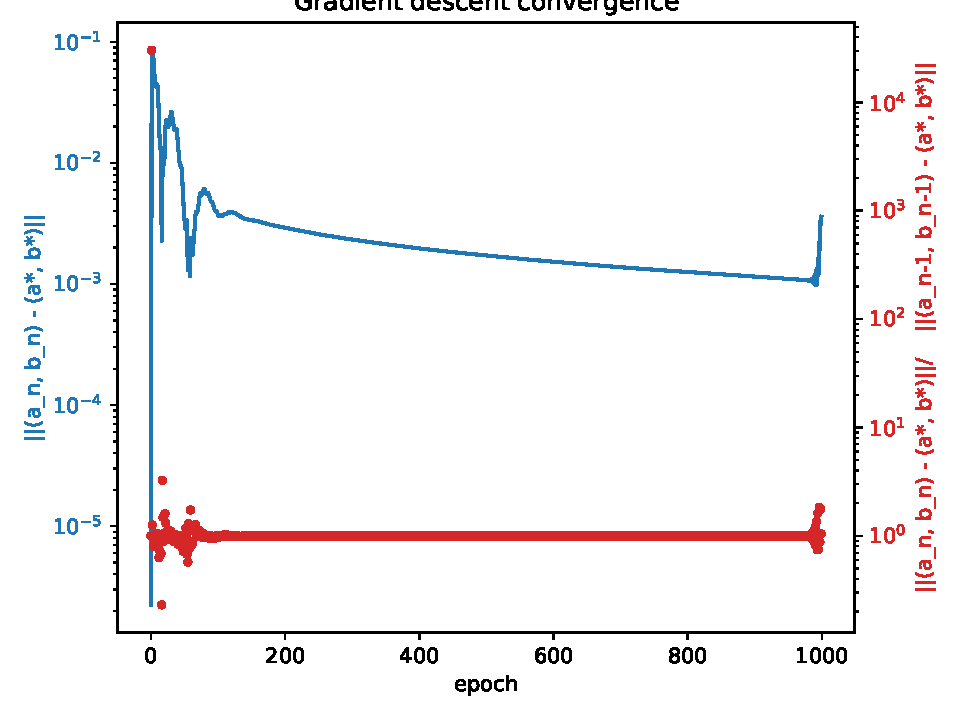
\includegraphics[width=\textwidth]{Homework1/ex2x2.pdf}
        \caption{AdamW}
    \end{subfigure}
    \centering
    \begin{subfigure}[t]{0.48\textwidth}
        \centering
        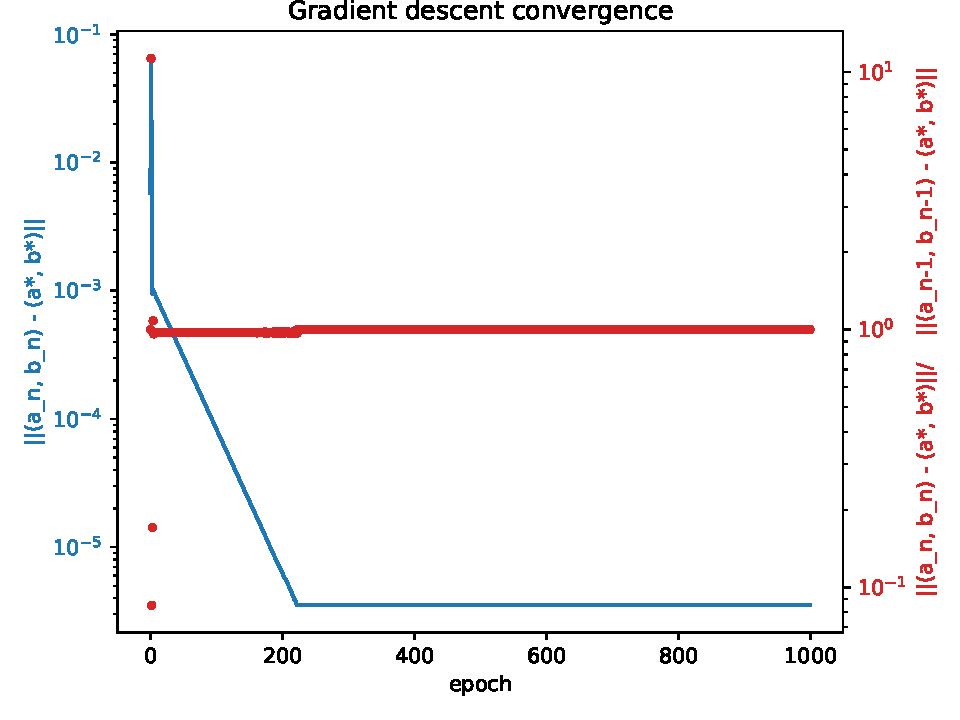
\includegraphics[width=\textwidth]{Homework1/ex2x3.pdf}
        \caption{Adagrad}
    \end{subfigure}
    \begin{subfigure}[t]{0.48\textwidth}
        \centering
        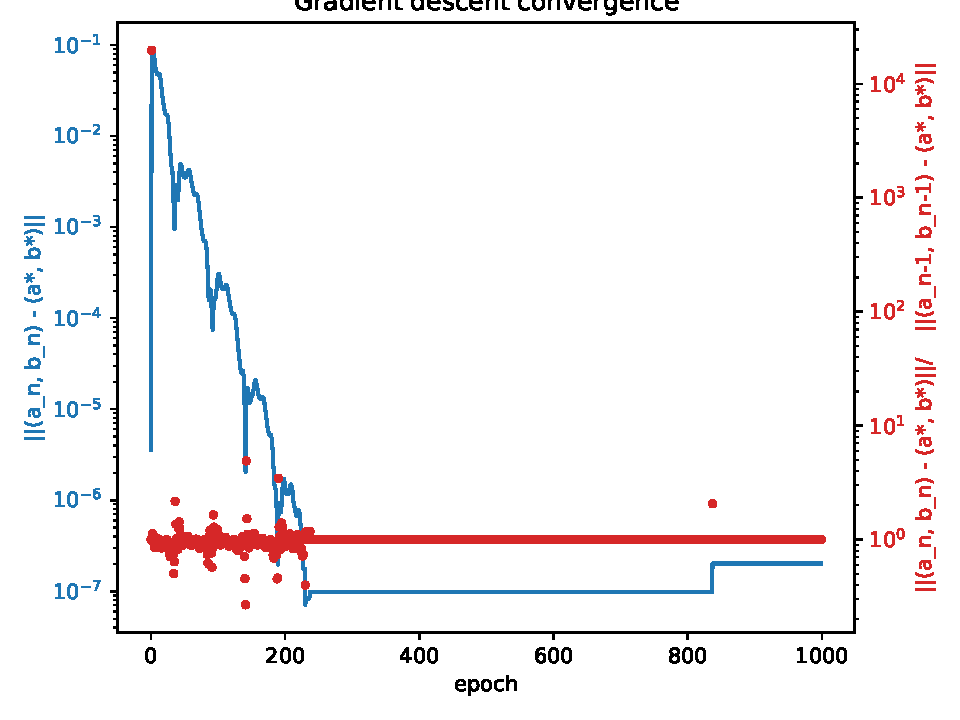
\includegraphics[width=\textwidth]{Homework1/ex2x4.pdf}
        \caption{Adamax}
    \end{subfigure}
    \centering
    \begin{subfigure}[t]{0.48\textwidth}
        \centering
        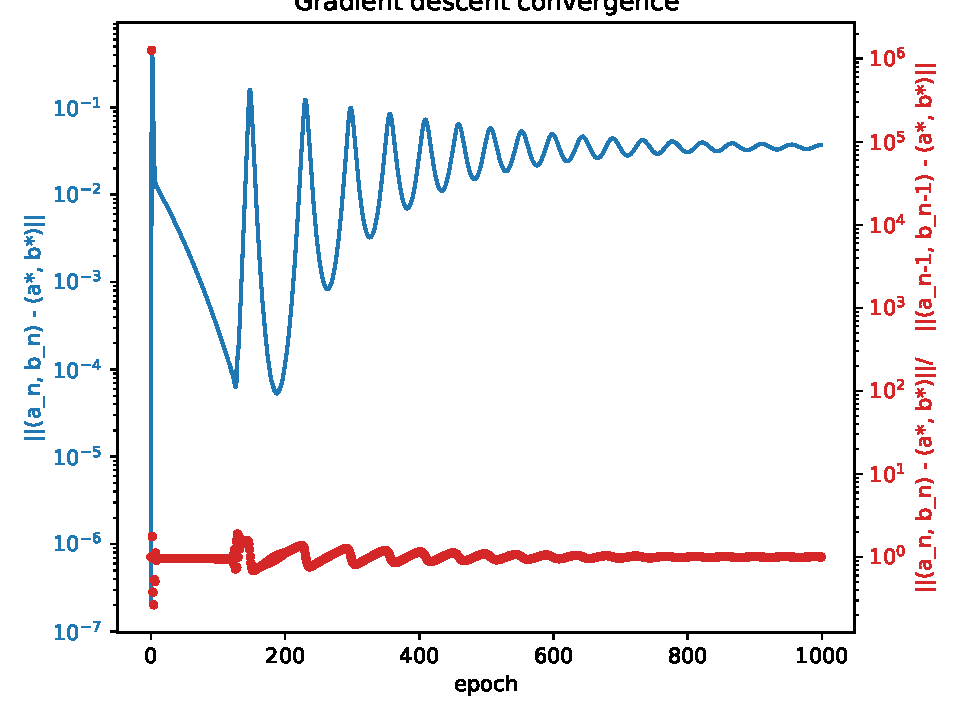
\includegraphics[width=\textwidth]{Homework1/ex2x5.pdf}
        \caption{RMSprop}
    \end{subfigure}
    \begin{subfigure}[t]{0.48\textwidth}
        \centering
        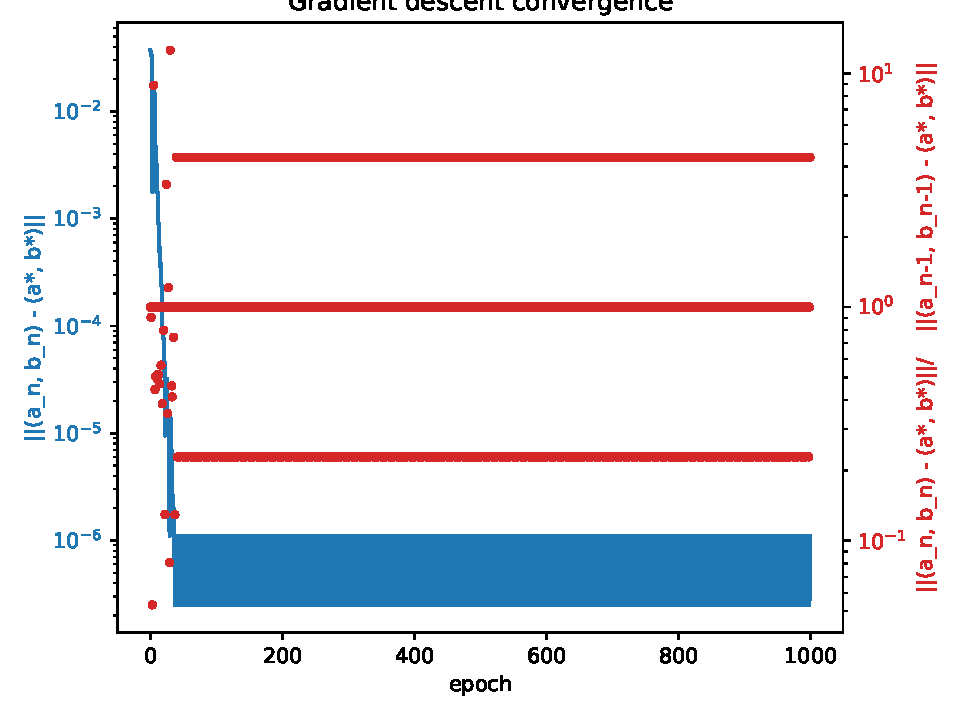
\includegraphics[width=\textwidth]{Homework1/ex2x6.pdf}
        \caption{Rprop}
    \end{subfigure}
\end{figure}
\inputminted[]{python}{./Homework1/ex2.py}

\subsection{Classification}
\begin{figure}[htbp]
    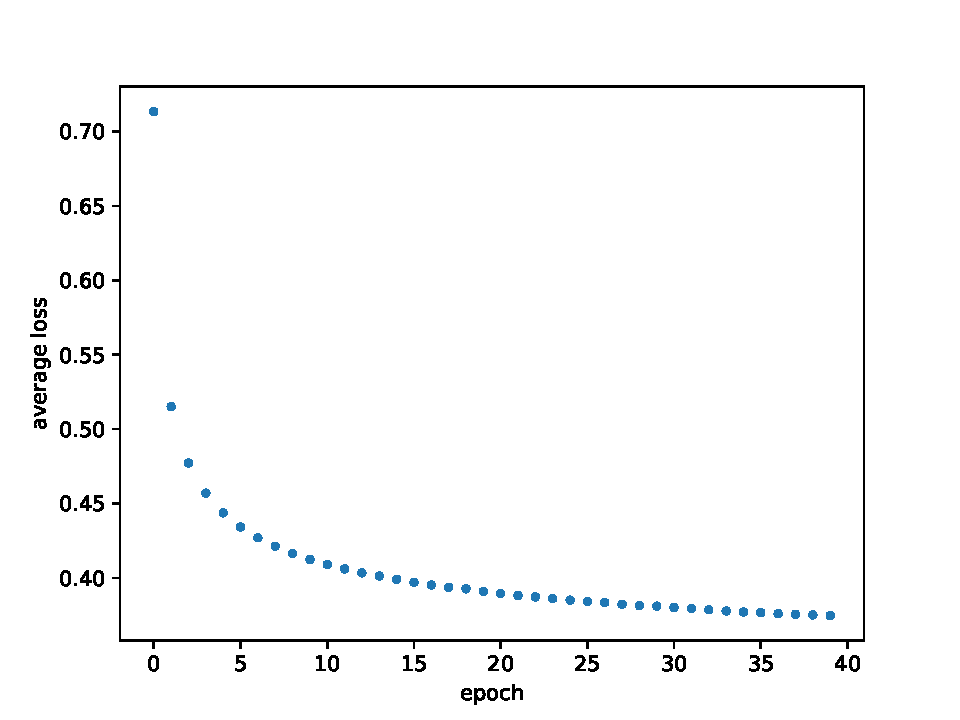
\includegraphics{Homework1/ex3b.pdf}
    \caption{Evolution of the loss}
\end{figure}
\foreach\x in {0,...,4}
{
\begin{figure}
\begin{center}
    \foreach \i in {{\number\numexpr2*\x\relax},{\number\numexpr2*\x+1\relax}}
    {
        \begin{subfigure}[p]{0.8\textwidth}
            \includegraphics[width=\textwidth]{Homework1/ex3c\i.pdf}
        \end{subfigure}
    }
\end{center}
\end{figure}
\clearpage
}
\inputminted[]{python}{./Homework1/ex3.py}


\end{document}